\documentclass{beamer}
\usepackage{graphicx}

\usetheme{Warsaw}
\definecolor{ulmcolor}{rgb}{0.33,0.41,0.47}
\usecolortheme[named=ulmcolor]{structure}

\title[Scikit-Learn]{Machine Learning with Scikit-Learn}
\author{Youssef Wally}
\institute{University Ulm}
\date{\today}




\begin{document}

\begin{frame}
\titlepage
\end{frame}

\begin{frame}{Training Models}
The idea is to find the least cost for the model. Meaning we want to find the value of theta that minimizes the cost function.
\end{frame}
\begin{frame}{Training Linear Regression Models}
The cost function for linear regression is its mean square root equation for theta. To find the theta that minimizes the cost function we use the normal equation:
\begin{equation}
\theta = (X^T X)^{-1}   X^T   y
\end{equation}
Where:
\begin{enumerate}
\item \( \theta \) is the value of \(\theta\)  that minimizes the cost function. 
\item  y is the vector of target values containing \( y^{1}\) to \(y^{m}\) .
\end{enumerate}
or SVD
\end{frame}
\begin{frame}
The problem is that computation of the normail equation is O(\(n^3\)) and O(\(n^2\)) for the SVD. Therefore there are different methods.
\end{frame}
\begin{frame}{Gradient descent}
The main idea is to start with a random \(\theta\) and then start changing it in order to minimize the cost function. An important thing to remember is that gradient descent works better when we scale the data. There are two types of gradient descent:
\begin{enumerate}
\item batch gradient descent
\item Stochastic gradient descent
\end{enumerate}
\end{frame}
\begin{frame}{Batch Gradient Descent}
The batch gradient descent considers the whole dataset. You then set the learning rate and number of iterations. However with large sets of data this will be slow
\end{frame}
\begin{frame}{Stochastic Gradient Descent}
Therefore Stochastic gradient descent uses one instance of the  data. This is benifical because its faster however it does not get the optiml theta but rather bounces around it.
\end{frame}
\begin{frame}{Mini-batch Gradient Descent }
Mini-batch Gradient Descent  makes a mix between both batch and Stochastic Gradient Descent by using samples of the data and not the whole set.
\end{frame}
\begin{frame}{summary}
\begin{figure}
\begin{center}
\centering
  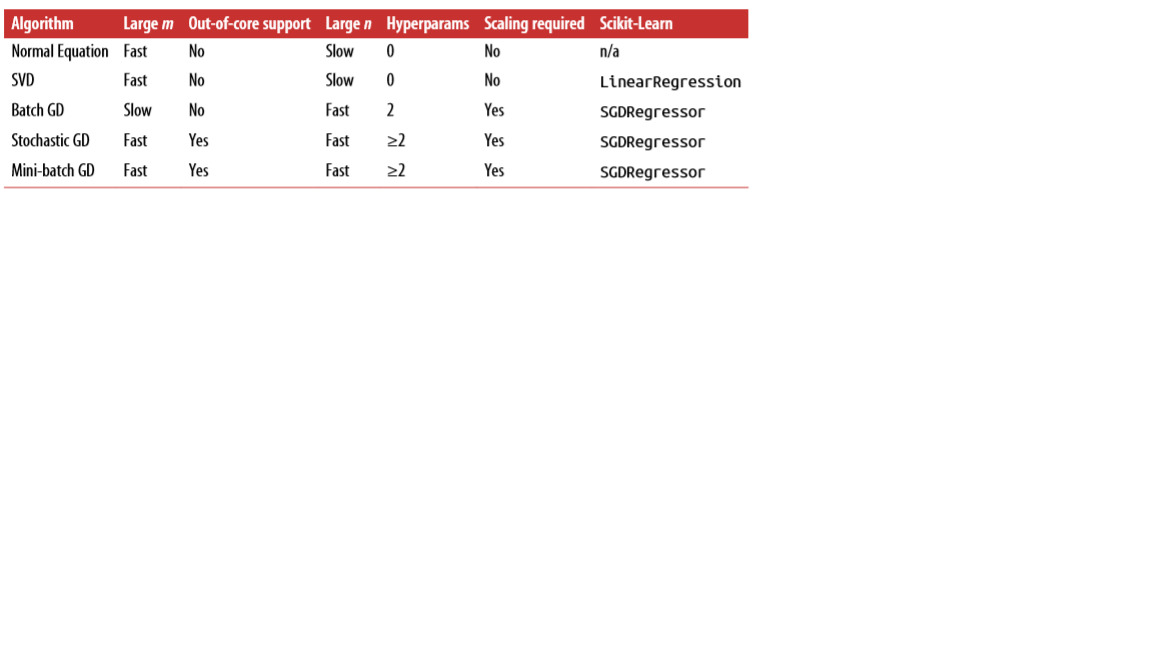
\includegraphics[totalheight=1\textheight]{Gradient Descent.png}
\end{center}
\end{figure}
\end{frame}

\begin{frame}{Polynomial Regression}
What if the data is non-linear? Then we can still use linear regression but add a polynomial feature and as its degree gets higher it fits better but it gets so high it will over fit. 
\begin{figure}
\begin{center}
\centering
  \includegraphics[totalheight=1\textheight]{Learning Curve.png}
\end{center}
\end{figure}
\end{frame}
\begin{frame}{Learning Curve}
A method to see the correctness of the model is the Learning curve.
\begin{figure}
\begin{center}
\centering
  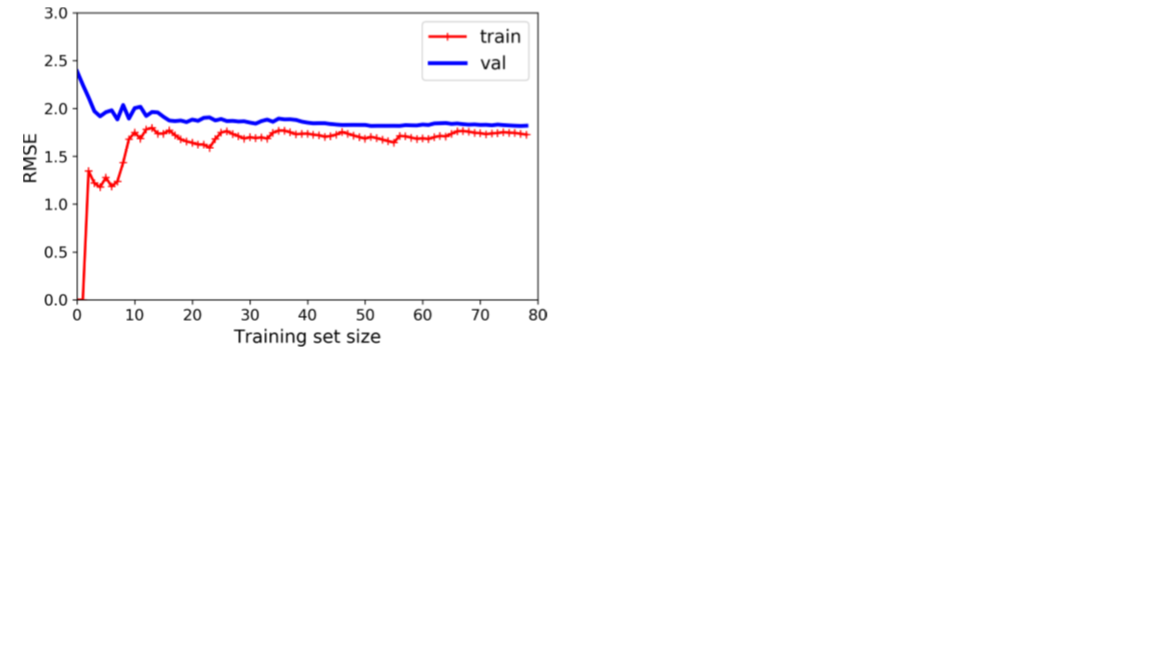
\includegraphics[totalheight=1\textheight]{Learning curve_trainval.png}
\end{center}
\end{figure}
\end{frame}
\begin{frame}{Bias}
This part of the generalization error is due to wrong assumptions, such as assuming that the data is linear when it is actually quadratic. A high-bias model is most likely to underfit the training data.10 
\end{frame}
\begin{frame}{Variance}
This part is due to the model’s excessive sensitivity to small variations in the training data. A model with many degrees of freedom (such as a high-degree polynomial model) is likely to have high variance, and thus to overfit the training data. 
\end{frame}
\begin{frame}{Regularized Linear Models}
Regularized models are linear regression but with small weight to allow small cost, For example:
\begin{enumerate}
\item Ridge Regression (searches for minimum weight)
\item Lasso Regression (tends to eliminate the weight of the least important feature)
\item Elastic Net (Mix of both depending on r)
\end{enumerate}
\end{frame}
\begin{frame}{Other methods for regularizing}
\begin{enumerate}
\item Early stopping; the method of just stopping when you have reached a minimum after awhile at it stayed the same for awhile 
\item Logistic Regression; a binary classifier if it is predeicted prob. is less than 50 percent then its true if not false, however there is no closed form for its gradient discent
\item softmax regression; using logistic regression to predict many classes but only mutually exclusive classes
\end{enumerate}
\end{frame}
\begin{frame}{SVM}
SVM can be used in linear/non linear classification, regression or detection
\begin{enumerate}
\item SVM is very feature sensitive
\end{enumerate}
\end{frame}
\begin{frame}{Linear SVM Classification}
Basically the separation of data by a straight line.
\begin{enumerate}
\item large margin classification is the fact of seperation the data with a line which is the furthest from the classified data to not be biased only on training data
\item however as the street goes wider the outliers increase the idea is to find the balance between hard and soft margin classification which is indicated with a number with the variable C
\end{enumerate}
\end{frame}
\begin{frame}{Nonlinear SVM Classification}
It is the same case as adding polynomial feature as we disscussed before or by a similarity function that takes many features and makes a landmark. However, it is slow as the degree increases. Thats why we use Polynomial Kernel or Gaussian RBF Kernel.
\begin{enumerate}
\item gamma makes bell shape narrower as it gets higher in Gaussian RBF Kernel
\end{enumerate}
\end{frame}
\begin{frame}{Summary}
\begin{figure}
\begin{center}
\centering
  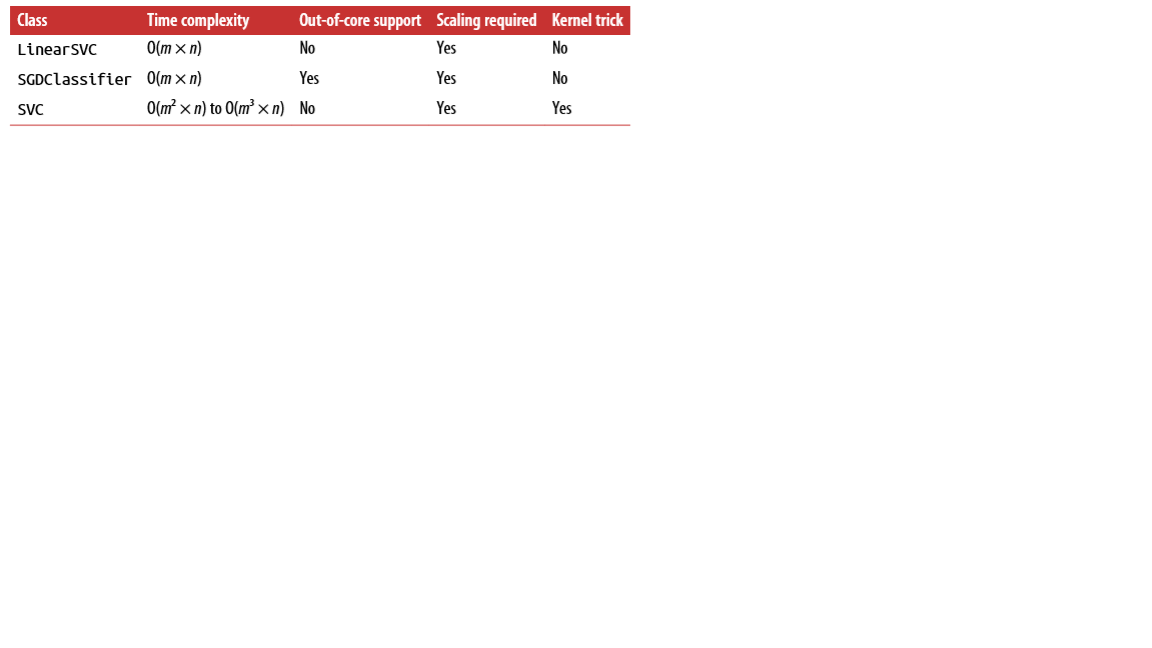
\includegraphics[totalheight=1.3\textheight]{Class_kernal.png}
\end{center}
\end{figure}
\end{frame}
\begin{frame}{SVM Regression}
The idea is to fit many data as possible on the line this time
\begin{enumerate}
\item epsilon determines the width of the 'street' (increase increase)
\end{enumerate}
and as always there is a kernal trick for the non linear regression.
\end{frame}
\begin{frame}{Decision Tress}
\begin{enumerate}
\item They are orthoganal and therefore rotation of data can cause problems, inaddition they are very sensitive so the same data can make two diffrent figures unless you set the random state (random forests takes average of trees and minimizes this)
\item Decision tress dont require scaling or centering
\item Samples: how many training sampeles are classified in that node
\item value: how much of the sample is in which class
\item gini: the purity of the class (classification)
\item MSE: mean square error, splits to minimize it (regression)
\end{enumerate}
\end{frame}

\end{document}